\setcounter{chapter}{1}
\setcounter{section}{0}
\setcounter{figure}{0}
\setcounter{equation}{0}
\setcounter{table}{0}
\chapter*{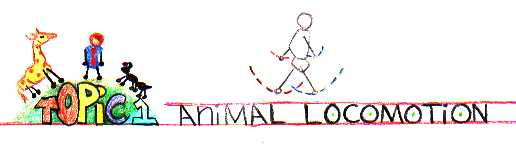
\includegraphics[width=\textwidth]{./figures/Topic1/Topic1.jpg}}
\addcontentsline{toc}{chapter}{Topic 1: Animal Locomotion}

\section{Introduction}

Imagine a giraffe, a Chihuahua, and an ant walking side by side without undue urgency. For every stride that the giraffe makes, the Chihuahua takes many and the ant many more. Most people intuitively know that the shorter the length of one’s legs, the faster they tend to swing. In other words, an inverse relation exists between the size of a creature and how quickly it can move its legs. Why would such a scaling relation exist?  
When walking at a leisurely pace, one may assume that the locomotion is executed in a way that minimizes energy expenditure.  A way to accomplish this is to let gravity do as much of the work whenever possible.  When an animal takes a step, the leg swings naturally from the hip, much like a pendulum in a gravitational field.  If the animal swings them faster or slower than their natural swinging time, you might think this may require undesirable additional energy expenditure. Thus, animals may want to swing their legs at precisely the natural swinging frequency of a pendulum in order to minimize energy expenditure. If so, does this account for why animals with shorter legs tend to swing them at a faster rate?  Let us set up the model and find out.

\section{Pendulum Motion}

\subsection{The Simple Pendulum: A Case in Point}

While almost any object can act as a pendulum, those that possess complex physical forms are difficult to analyze.  For this reason, we will begin by examining the most straightforward case: the simple pendulum in a gravitational field.  The simple pendulum is aptly named, for it simply consists of a point mass suspended from a massless string.  The string is made massless to avoid having to calculate its rotational inertia, which, as you may recall, is a quantity that depends on the distribution of mass.  If we think of the leg as a simple pendulum, it is as if the entire mass of the leg is concentrated in the foot.  Figure \ref{Fig1-1} below shows a simple pendulum of length $\ell$ and mass $m$.  As the pendulum oscillates, the point mass traces an arc of the circle of radius $\ell$.
\begin{figure}[htb]
\centering
	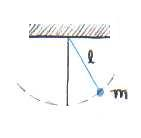
\includegraphics[width=2.5in]{./figures/Topic1/Figure1-1.jpg}
	\caption{The simple pendulum with length $\ell$ and mass $m$.}
	\label{Fig1-1}
\end{figure}

 
We are now ready to derive an equation that describes the position of the pendulum as a function of time.  From the equation, we will then obtain another equation that computes the stepping time for an animal.  
What are the forces acting on the mass?  The best way to visualize them is by drawing a force diagram (Figure~\ref{Fig1-2}).  
\begin{figure}[htb]
	\centering
	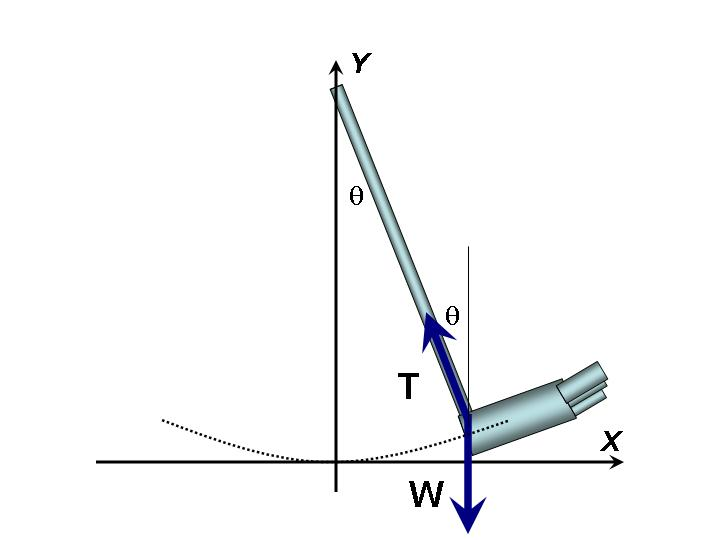
\includegraphics[width=3.0in]{./figures/Topic1/Figure1-2.jpg}
	\caption{Free-body diagram for mass m.}
	\label{Fig1-2}
\end{figure}

According to Newton’s 2nd Law, the sum of the forces along the $x$-axis and $y$-axis are equal to the mass, $m$, multiplied by the acceleration in the $x$-direction, $a_x$, and in the $y$-direction, $a_y$, respectively.
$$\sum F_x = ma_x$$
$$\sum F_y = ma_y$$
To simplify the problem, we will assume that the movement of the foot along the $y$-direction is always negligible compared to the one along the $x$-direction. This is approximately true when taking moderate steps, for which the angle $\theta$ rarely exceeds 20$^{\circ}$. If so, we may also ignore the acceleration of the foot along the $y$ when we invoke Newton’s second law. When taking this into account, and breaking down the forces into $x$ and $y$ components as shown in Fig.~\ref{Fig1-3}, we obtain 
\begin{figure}[htb]
	\centering
	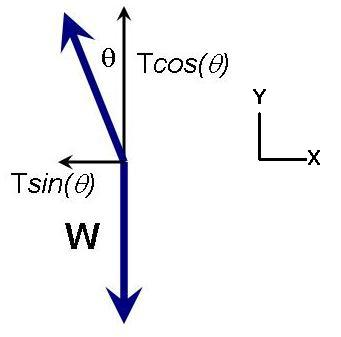
\includegraphics[width=2.5in]{./figures/Topic1/Figure1-3.jpg}
	\caption{Force diagram, with the tension, $T$, broken down into its $x$ and $y$ components.}
	\label{Fig1-3}
\end{figure} 

\begin{equation}\label{eqn1-1}
\sum F_x = T \sin\left(\theta\right) = ma_x
\end{equation}
\begin{equation}\label{eqn1-2}
\sum F_y = -w + T \cos\left(\theta\right) = 0
\end{equation}
When Eq.~\ref{eqn1-2} is solved for the tension ($T = w/ \cos(\theta)$), and this expression is substituted for $T$ in Eq.~\ref{eqn1-1}, we derive the following relation between $a_x$ and the weight 
\begin{eqnarray}\label{eqn1-3}
ma_x = -\frac{w}{\cos\left(\theta\right)} \sin\left(\theta\right) = -w \tan\left(\theta\right)
\end{eqnarray}

Since $w=mg$, we can simplify:
$$ma_x = -mg \tan\left(\theta\right)$$       
\begin{eqnarray}\label{eqn1-4}
a_x = -g \tan\left(\theta\right)             
\end{eqnarray}
Note that the acceleration is not constant, that is, it varies with the angle $\theta$, which is dependent on the position $x$ of the foot along the horizontal. Hence we cannot use simple approaches like the kinematic equations to solve for the time it takes to complete a step.  We will approach the solution to Eq.~\ref{eqn1-4} differently than what is done in an introductory physics course. 
Recall that the tangent of an angle can be defined as the ratio of the opposite and adjacent sides of a right triangle.
$$\tan\left(\theta\right)  = \frac{{\rm opposite}}{{\rm adjacent}}$$
In our case, as shown below in Fig.~\ref{Fig1-4}, the adjacent of angle $\theta$ is simply the length of the leg $\ell$. 
\begin{figure}[htb]
	\centering
	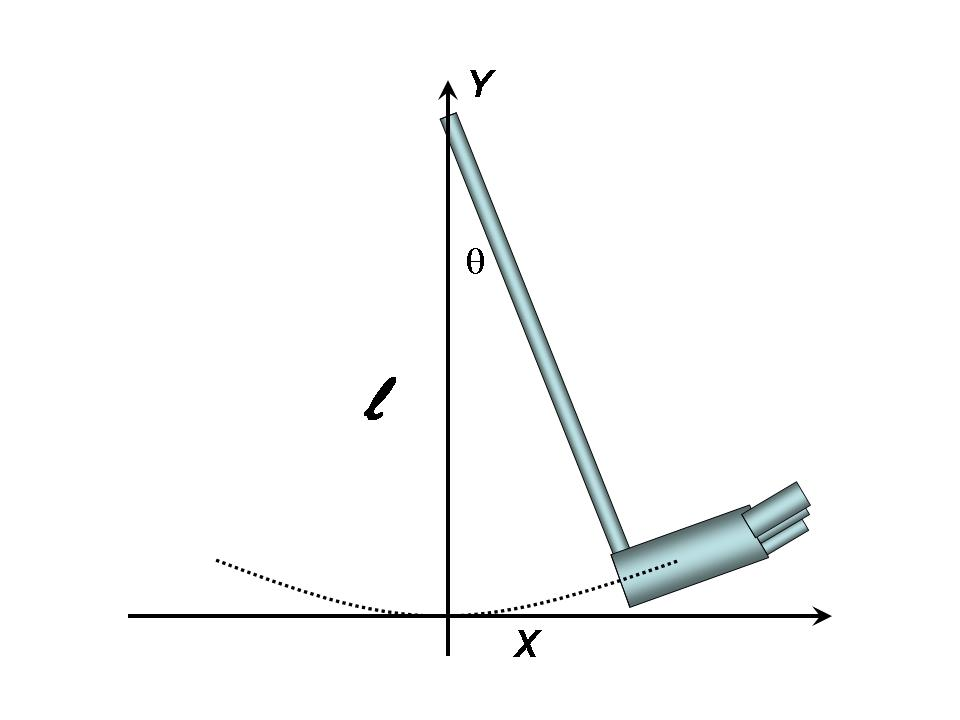
\includegraphics[width=2.5in]{./figures/Topic1/Figure1-4.jpg}
	\caption{Adjacent and opposite sides of the triangle defined by $\theta$.}
	\label{Fig1-4}
\end{figure} 
The opposite here corresponds to the displacement of the foot, or $x$, along the x-direction. Accordingly, $\tan\left(\theta\right) \approx x/l$, and Eq.~\ref{eqn1-4} becomes:
\begin{eqnarray}\label{eqn1-5}
a_x = -\frac{g}{\ell}x
\end{eqnarray}             
But ax also varies with position and time.  Recall that velocity is the first derivative of position with respect to time and that acceleration is the first derivative of velocity with respect to time.  It follows that acceleration is the second derivative of position with respect to time, written in differential form as:
\begin{eqnarray}\label{eqn1-6}
a_x = \frac{d^2x}{dt^2}
\end{eqnarray}      
Substituting Eq.~\ref{eqn1-4} into Eq.~\ref{eqn1-5}, we arrive at the equation we must solve for $x$:
\begin{eqnarray}\label{eqn1-7}
\frac{d^2x}{dt^2} = -\frac{g}{\ell}x
\end{eqnarray} 
Eq.~\ref{eqn1-7} is of a type known as a ``differential equation'' because it contains a derivative of what you solving for. Since solving differential equations is beyond the scope of the course, the steps are left to the more ambitious student.  However, as you will verify in one of your homework problems, the following solutions satisfy Eq.~\ref{eqn1-7}.
\begin{eqnarray}\label{eqn1-8}
x = A \sin\left(\sqrt{\frac{g}{\ell}}~t\right)
\end{eqnarray}
or
\begin{eqnarray}\label{eqn1-9}
x = A \cos\left(\sqrt{\frac{g}{\ell}}~t\right),
\end{eqnarray}
where $A$ is a constant. \footnote[1]{The procedure is quite simple.  To verify for example that Eq.~\ref{eqn1-8} is a solution, first take the second derivative of the right hand side. Then show that with some algebraic manipulation that it equals $-(g/l)x$ as Eq.~\ref{eqn1-7} suggests.}

The constant, $A$, in each case refers to the amplitude of the step, and we can visualize the motion in terms of its oscillatory behavior, shown in Figure\ref{Fig1-5}.
\begin{figure}[htb]
	\centering
	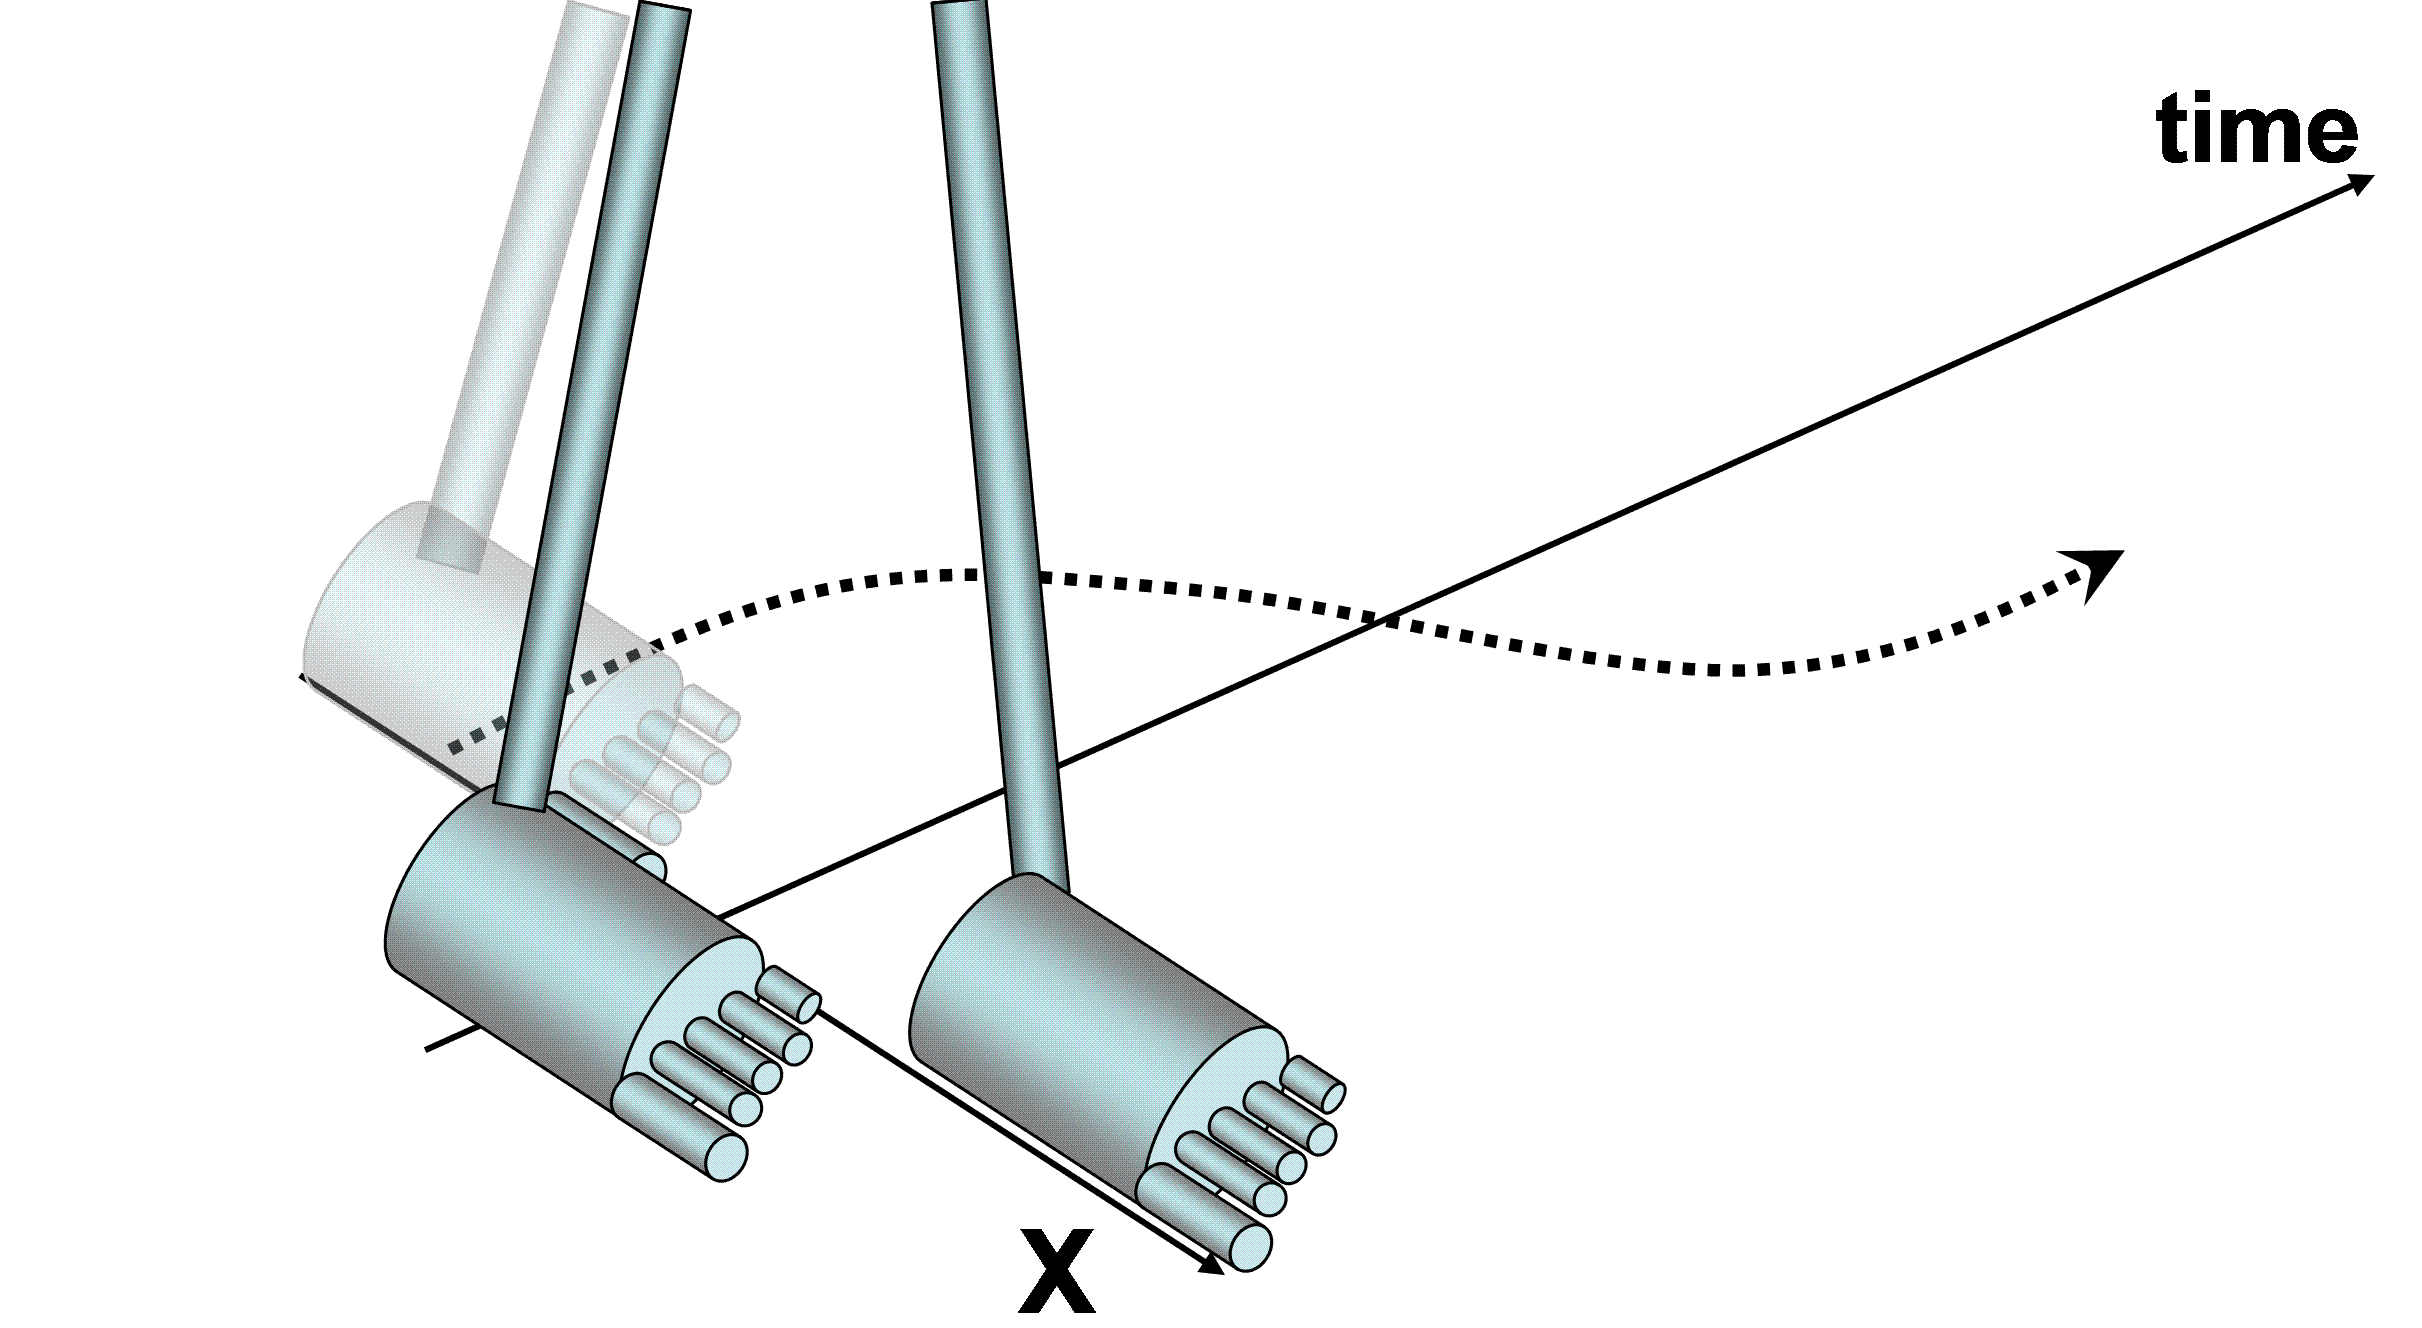
\includegraphics[width=2.25in]{./figures/Topic1/Figure1-5a.png}
	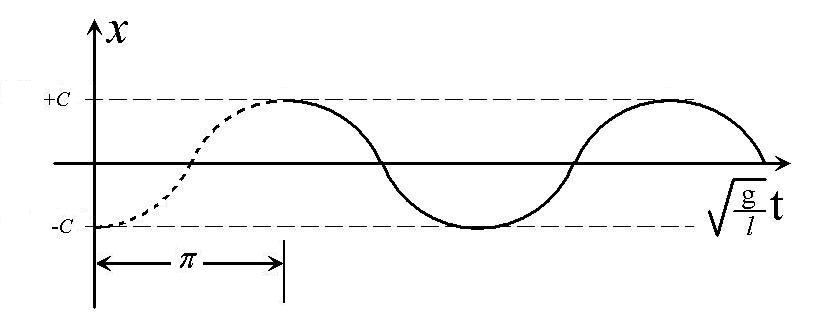
\includegraphics[width=3.25in]{./figures/Topic1/Figure1-5b.png}
	\caption{As the back leg moves forward it undergoes motion corresponding to half of a full pendulum oscillation.}
	\label{Fig1-5}
\end{figure}
From Fig.\ref{Fig1-5} we see that a step corresponds to one half of the full sinusoidal oscillation. In terms of our solutions Eq~\ref{eqn1-8} and Eq.~\ref{eqn1-9}, this corresponds to a time such that 
\begin{eqnarray}\label{eqn1-10}
\pi = \sqrt{\frac{g}{\ell}}\tau
\end{eqnarray}
Solving for $\tau$, we get the theoretical time it takes for the leg to step forward:
\begin{eqnarray}\label{eqn1-11}
\tau = \pi\sqrt{\frac{\ell}{g}}
\end{eqnarray}
Interestingly enough, in this model, the mass of the body or leg does not affect how long it takes for an animal to take a step; only the leg length and the magnitude of gravity are determining factors.  Note that the stepping time $\tau$ varies with the square root of $\ell$, proving that our intuition is correct—longer legs do require more time to take a step.

How accurately does Eq.~\ref{eqn1-11} predict stepping time?  The leg of the average adult human is approximately 0.9 m, corresponding to a theoretical stepping time of 0.95 s.  Biophysics students measure $\tau$ as part of a laboratory activity, finding it to be closer to 0.6-0.7 s.  The error is about 50\%, which is relatively small when one considers that the human leg looks nothing like a point mass attached to a massless string.  In the next section, we will improve the model by taking into account the distribution of mass in the leg.  

\subsection{The Physical Pendulum: A Refined Model}

Contrasted with the simple pendulum where the mass is concentrated at a point, the physical pendulum approach is capable of handling any arbitrary distribution of mass that swings about a fixed pivot.  Examine the diagram shown below for a human leg swinging as a physical pendulum.
\begin{figure}[htb]
	\centering
	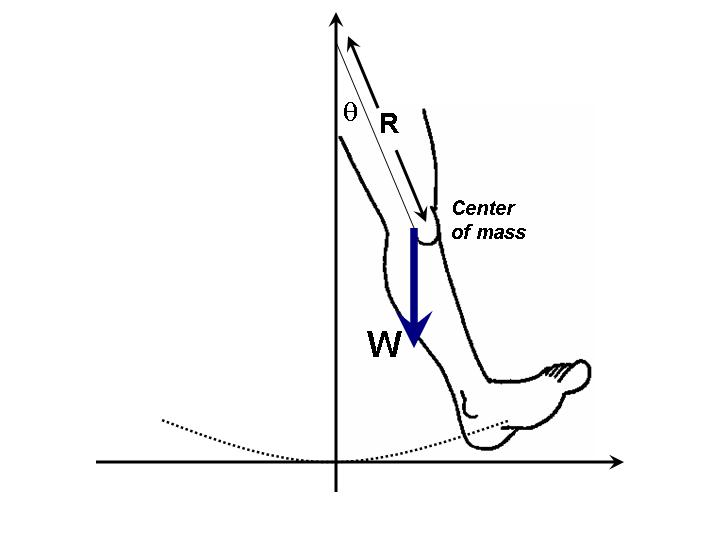
\includegraphics[width=3.5in]{./figures/Topic1/Figure1-6.jpg}
	\caption{Free body diagram of the physical pendulum.}
	\label{Fig1-6}
\end{figure}
  
A significant difference between the simple pendulum and the physical pendulum models is that the first looks at the action of forces, whereas the second focuses on torques. Recall that a torque is the turning force that causes objects to rotate about a pivot point. The strength of the torque is dependent not only on the applied force but also on distance from where it is applied to the pivot point. In this case, gravity is the only force that causes rotational motion, and the magnitude of the torque associated with this force is the force $F$ times the distance from where it is applied to the pivot point ($R$). In addition, the product must be multiplied by the sine of the angle between the directions of the force and the line of action which connects the pivot point to the center of mass. The resulting expression is $w R \sin\theta$, or $m g R \sin\theta$, where $R$ is the distance from the pivot point to the center of mass.  Note that in Fig.~\ref{Fig1-6} the direction of the torque (clockwise) opposes the angular displacement $\theta$ (counter-clokwise). This is always the case, even if the leg is to the left of the centerline; in that case the direction of the angular displacement is clockwise whereas that of the torque is counter-clockwise. 
The sum of the torques acting on the mass obeys the equation
\begin{eqnarray}\label{eqn1-12}
\sum \tau = I\alpha
\end{eqnarray}
where $\tau$ is now defining torque rather than a characteristice time, $I$ is the moment of inertia and $\alpha$ is the angular acceleration.  Recall that the moment of inertia takes into account the distribution of mass of the leg.  In fact, if you divide the leg into small masses, and identify each mass $m$ with an index $n$, the moment of inertia is given by the formula  $$I=\sum_n m_n R_n^2.$$  
Angular acceleration, $\alpha$ is the second derivative of $\theta$ with respect to time.  Thus, Eq.~\ref{eqn1-12} can be rewritten as
\begin{eqnarray}\label{eqn1-13}
-R m g \sin\left(\theta\right)=I\frac{d^2\theta}{dt^2}
\end{eqnarray}
Rearranging, we get:
\begin{eqnarray}\label{eqn1-14}
\frac{d^2\theta}{dt^2} = -\frac{Rmg}{I}\sin\theta
\end{eqnarray}
As we stated earlier, an animal’s leg rarely subtends an angle greater than 20$^{\circ}$ relative to the normal while walking.  This means that that we can take advantage of the small angle approximation, which states that for angles less than 20$^{\circ}$, $\sin\theta \approx \theta$.  (Recall that the small angle approximation only holds when the angle is expressed in radians.)  Eq.~\ref{eqn1-14} simplifies to
\begin{eqnarray}\label{eqn1-15}
\frac{d^2\theta}{dt^2} = -\frac{RMg}{I}\theta
\end{eqnarray}
Compare Eq.~\ref{eqn1-7} to Eq.~\ref{eqn1-15}.  Instead of $x$, we now have $\theta$, and instead of the constant $g/\ell$, we now have $Rmg/I$.  Observing these substitutions makes solving Eq.~\ref{eqn1-15} easy, because we have already solved Eq.~\ref{eqn1-7}. The solutions are of the form: 
\begin{eqnarray}\label{eqn1-16}
\theta(t) = A \sin\left(\sqrt{\frac{Rmg}{I}}t\right)
\end{eqnarray}
or
\begin{eqnarray}\label{eqn1-17}
\theta(t) = A \cos\left(\sqrt{\frac{Rmg}{I}}t\right)
\end{eqnarray}
Also analogous to the previous case, a step corresponds to the time when the period is 
\begin{eqnarray}\label{eqn1-18}
\pi = \sqrt{\frac{Rmg}{I}}t
\end{eqnarray}
and the stepping time is
\begin{eqnarray}\label{eqn1-19}
\tau = \pi\sqrt{\frac{I}{Rmg}}
\end{eqnarray}
As stated above, the moment of inertia $I$ of an object pivoting about an axis is found by first breaking down the object into small pieces each with the same mass $m$. After identifying each mass $m$ with an index $n$, the moment of inertia is given by the formula $I=\sum_n m_nR_n^2$.   Most physics textbooks list the result of this calculation for the moments of inertia of various bodies with simple geometries. To take advantage of these existing formulas for $I$, we can assume a simplified shape for the leg by thinking of it as a slender rod with a pivot through one end (the hip).  Accordingly, 
$$I=\frac{1}{3}m\ell^2$$
$$R = \frac{1}{2}\ell$$
where $\ell$ is the length of the leg and $m$ is the total mass of the leg. If we substitute these equations into Eq.~\ref{eqn1-19}, we get an equation that calculates the stepping time, accounting for the continuous mass distribution of the leg.
\begin{eqnarray}\label{eqn1-20}
\tau = \pi\sqrt{\frac{2\ell}{3g}}
\end{eqnarray}
This equation is almost identical to Eq.~\ref{eqn1-11} for the simple pendulum case, with the exception of a new constant, $\sqrt{2/3}$, which is approximately 0.8.  The new factor makes the theoretical stepping time $\tau$ = 0.78 s, which is about 20\% lower than when computed using the simple pendulum model.  Now the theoretical time more closely matches the experimental measurements for adult humans, which was in the range of 0.6 to 0.7 s.

One might be tempted to think that leg length is the only variable that affects the stepping time.  However, $\tau$ is just as dependent on the gravitational constant.  Eq.~\ref{eqn1-20} explains why astronauts move differently on the moon, where $g$ is about 1/6 of Earth’s value.  Because of the diminished $g$, each step takes about 2.5 (or $\sqrt{6}$) times as long as on Earth. The increased stepping time apparently became unbearably long for these astronauts, who immediately found that to get from point A to point B quickly, it was more efficient to hop than to walk.  This incident also underscores how our bodies have adapted to the gravitational environment in which we live.